\documentclass[11pt,a4paper,titlepage]{article}
\usepackage[a4paper]{geometry}
\usepackage[utf8]{inputenc}
\usepackage[english]{babel}
\usepackage{lipsum}
\usepackage{eurosym}
\usepackage{rotating}

\usepackage{amsmath, amssymb, amsfonts, amsthm, mathtools}
% mathtools for: Aboxed (put box on last equation in align envirenment)
\usepackage{microtype} %improves the spacing between words and letters

\usepackage{lipsum}
\usepackage{threeparttable}
\usepackage{tabularx}
\usepackage{multirow}
\usepackage{booktabs}
\newcommand{\tabitem}{~~\llap{\textbullet}~~}
\usepackage{graphicx}
\graphicspath{ {./figures/} {./eps/}}
\usepackage{epsfig}
\usepackage{epstopdf}
\usepackage{verbatim}
\usepackage{textcomp}
\usepackage{tikz}
\usetikzlibrary{shapes,arrows}

%%%%%%%%%%%%%%%%%%%%%%%%%%%%%%%%%%%%%%%%%%%%%%%%%%
%% COLOR DEFINITIONS
%%%%%%%%%%%%%%%%%%%%%%%%%%%%%%%%%%%%%%%%%%%%%%%%%%
 % Enabling mixing colors and color's call by 'svgnames'
%%%%%%%%%%%%%%%%%%%%%%%%%%%%%%%%%%%%%%%%%%%%%%%%%%
\definecolor{MyColor1}{HTML}{CC0000} %mix personal color
\newcommand{\textb}{\color{Black} \usefont{OT1}{lmss}{m}{n}}
\newcommand{\blue}{\color{MyColor1} \usefont{OT1}{lmss}{m}{n}}
\newcommand{\blueb}{\color{MyColor1} \usefont{OT1}{lmss}{b}{n}}
\newcommand{\red}{\color{LightCoral} \usefont{OT1}{lmss}{m}{n}}
\newcommand{\green}{\color{Turquoise} \usefont{OT1}{lmss}{m}{n}}
%%%%%%%%%%%%%%%%%%%%%%%%%%%%%%%%%%%%%%%%%%%%%%%%%%


%%%%%%%%%%%%%%%%%%%%%%%%%%%%%%%%%%%%%%%%%%%%%%%%%%
%% FONTS AND COLORS
%%%%%%%%%%%%%%%%%%%%%%%%%%%%%%%%%%%%%%%%%%%%%%%%%%
%    SECTIONS
%%%%%%%%%%%%%%%%%%%%%%%%%%%%%%%%%%%%%%%%%%%%%%%%%%
\usepackage{titlesec}
\usepackage{sectsty}
%%%%%%%%%%%%%%%%%%%%%%%%
%set section/subsections HEADINGS font and color
\sectionfont{\color{MyColor1}}  % sets colour of sections
\subsectionfont{\color{MyColor1}}  % sets colour of sections

%set section enumerator to arabic number (see footnotes markings alternatives)
\renewcommand\thesection{\arabic{section}.} %define sections numbering
\renewcommand\thesubsection{\thesection\arabic{subsection}} %subsec.num.

%define new section style
\newcommand{\mysection}{
\titleformat{\section} [runin] {\usefont{OT1}{lmss}{b}{n}\color{MyColor1}}
{\thesection} {3pt} {} }

%%%%%%%%%%%%%%%%%%%%%%%%%%%%%%%%%%%%%%%%%%%%%%%%%%
%		CAPTIONS
%%%%%%%%%%%%%%%%%%%%%%%%%%%%%%%%%%%%%%%%%%%%%%%%%%
\usepackage{caption}
\usepackage{subcaption}
%%%%%%%%%%%%%%%%%%%%%%%%
\captionsetup[figure]{labelfont={color=MyColor1}}

%%%%%%%%%%%%%%%%%%%%%%%%%%%%%%%%%%%%%%%%%%%%%%%%%%
%		!!!EQUATION (ARRAY) --> USING ALIGN INSTEAD
%%%%%%%%%%%%%%%%%%%%%%%%%%%%%%%%%%%%%%%%%%%%%%%%%%
%using amsmath package to redefine eq. numeration (1.1, 1.2, ...)
%%%%%%%%%%%%%%%%%%%%%%%%
\renewcommand{\theequation}{\thesection\arabic{equation}}

%set box background to grey in align environment
\usepackage{etoolbox}% http://ctan.org/pkg/etoolbox
\makeatletter
\patchcmd{\@Aboxed}{\boxed{#1#2}}{\colorbox{black!15}{$#1#2$}}{}{}%
\patchcmd{\@boxed}{\boxed{#1#2}}{\colorbox{black!15}{$#1#2$}}{}{}%
\makeatother
%%%%%%%%%%%%%%%%%%%%%%%%%%%%%%%%%%%%%%%%%%%%%%%%%%

\newcommand{\DP}[1]{\textcolor{blue}{\textbf{(DP says: #1)}}}
\newcommand{\cri}[1]{\textcolor{green}{\textbf{(Cri says: #1)}}}

\makeatletter
\let\reftagform@=\tagform@
\def\tagform@#1{\maketag@@@{(\ignorespaces\textcolor{red}{#1}\unskip\@@italiccorr)}}
\renewcommand{\eqref}[1]{\textup{\reftagform@{\ref{#1}}}}
\makeatother
\usepackage[hidelinks]{hyperref}

%% LISTS CONFIGURATION %%
\usepackage{enumitem}
\setlist[enumerate,1]{start=0}
\renewcommand{\labelenumii}{\theenumii}
\renewcommand{\theenumii}{\theenumi.\arabic{enumii}.}

\usepackage[acronym]{glossaries}
\newacronym[plural=GEO,longplural={Geostationary Earth Orbits}]{geo}{GEO}{Geostationary Earth Orbit}
\newacronym[plural=LEO,longplural={Low Earth Orbits}]{leo}{LEO}{Low Earth Orbit}
\newacronym[plural=MEO,longplural={Medium Earth Orbits}]{meo}{MEO}{Medium Earth Orbit}
\newacronym[plural=HEO,longplural={High Elliptical Orbits}]{heo}{HEO}{High Elliptical Orbit}
\newacronym{eci}{ECI}{Earth Centered Inertial}
\newacronym{lla}{LLA}{geodetic latitude, longitude, altitude coordinates}
\newacronym[plural=GS,longplural={Ground Stations}]{gs}{GS}{Ground Station}
\newacronym{raan}{RAAN}{Right Ascending of Ascension Node}
\newacronym{eirp}{EIRP}{Effective Isotropic Radiated Power}
\newacronym{eol}{EOL}{End Of Life}

%%%%%%%%%%%%%%%%%%%%%%%%%%%%%%%%%%%%%%%%%%%%%%%%%%
%% PREPARE TITLE
%%%%%%%%%%%%%%%%%%%%%%%%%%%%%%%%%%%%%%%%%%%%%%%%%%
\title{\blue Eytu project}
\author{Davide Peron\\ Cristina Gava}
\date{\today}
%%%%%%%%%%%%%%%%%%%%%%%%%%%%%%%%%%%%%%%%%%%%%%%%%%

\begin{document}
\maketitle

\tableofcontents
\clearpage

\section{Power supply}
  \subsection{Wii U main console}
      On the Wii U motherboard there is a discrete number of components involved in the power supply section, there are both passive components, discrete semiconductors and Integrated circuits all working together to power the PCB. In \autoref{tab:power} we summarized the main components listed under type and name: we can see the huge amount of passive components needed to support the integrated circuits and the discrete amount of transistors and      diodes; on the other hand the number of integrated circuit is restrained.

      In figure \autoref{fig:motherboard} a photo of the motherboard section regarding the power supply is shown: the red squares represent three N-channel MOSFET, used to minimize losses in power conversion. Since one of their applications is for a rectifier in DC/DC converters, we suppose they are part of the power supply system in the board \cite{mosfet8026}.

      \begin{figure}
        \centering
        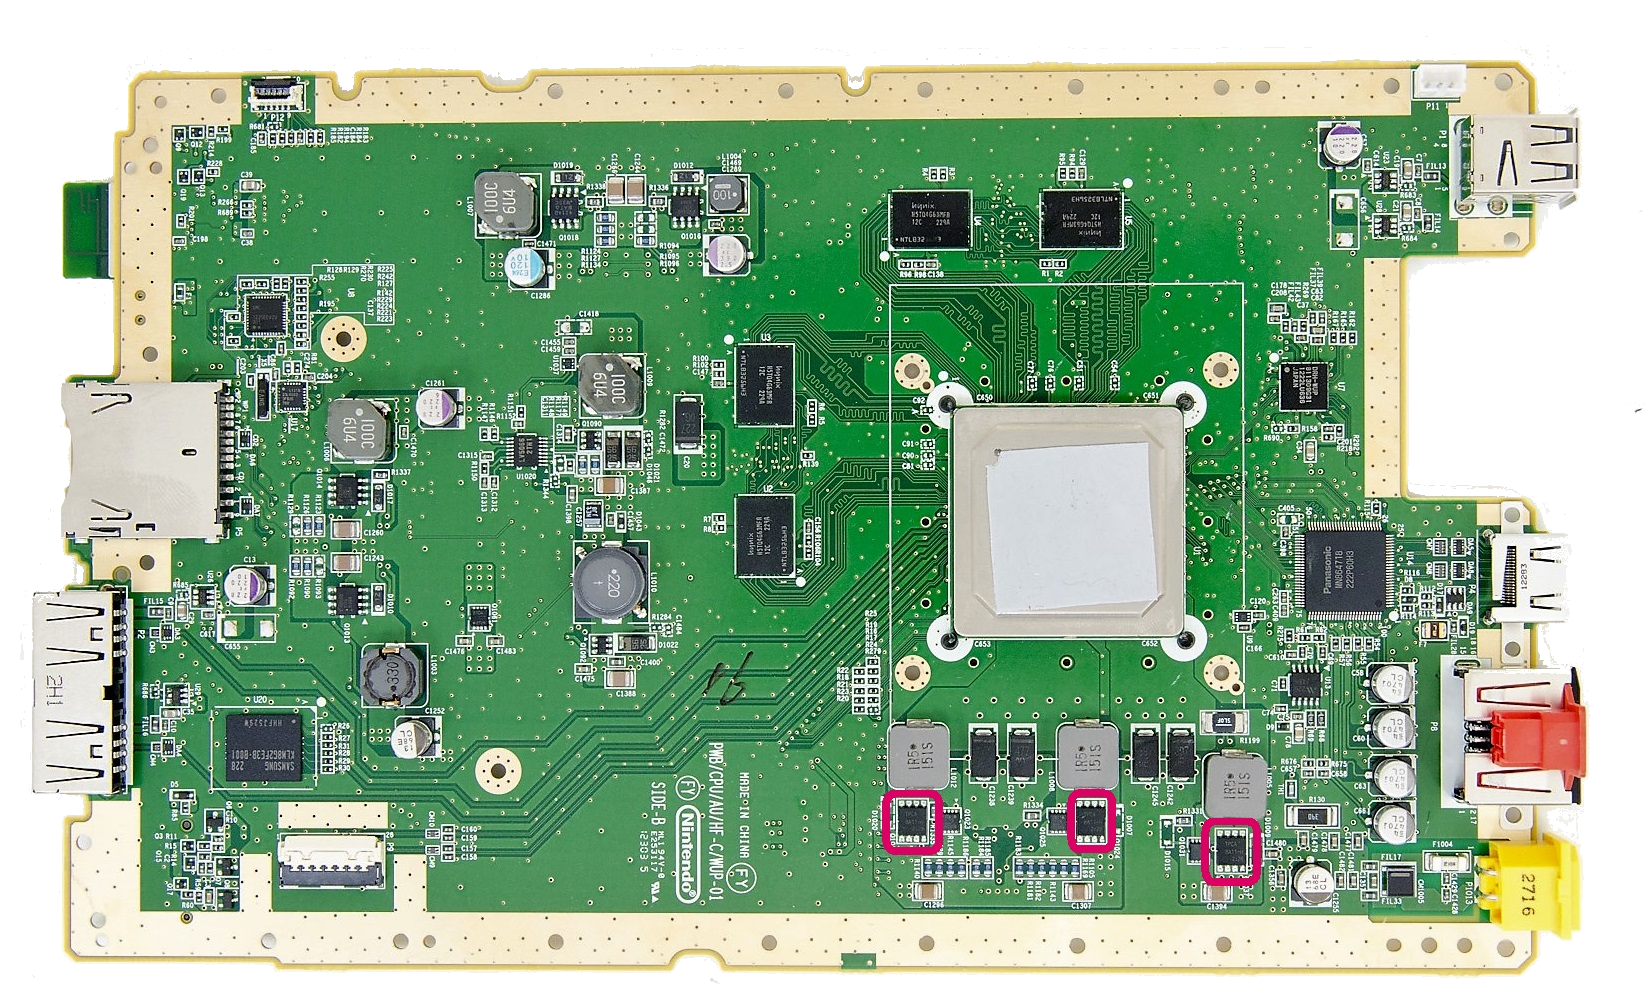
\includegraphics[width = .85\textwidth]{motherboard_front.png}
        \caption{Motherboard front part (power section)}
        \label{fig:motherboard}
      \end{figure}

      \subsubsection{Integrated circuits description}
        The three main integrated components that are worth to be described are:
        \begin{itemize}
          \item \textit{The power management IC}, model TPS65070RSL from Texas Instruments;
          \item \textit{The Regulator DC/DC Converter, Step-Up}, model AIC1634GG from Analog Integration corp.;
          \item \textit{The switching Regulator DC/DC Controller, Step-Down}, model LV5066V from ON Semiconductors.
        \end{itemize}

        \begin{figure}
          \begin{minipage}{.5\textwidth}
          \centering
          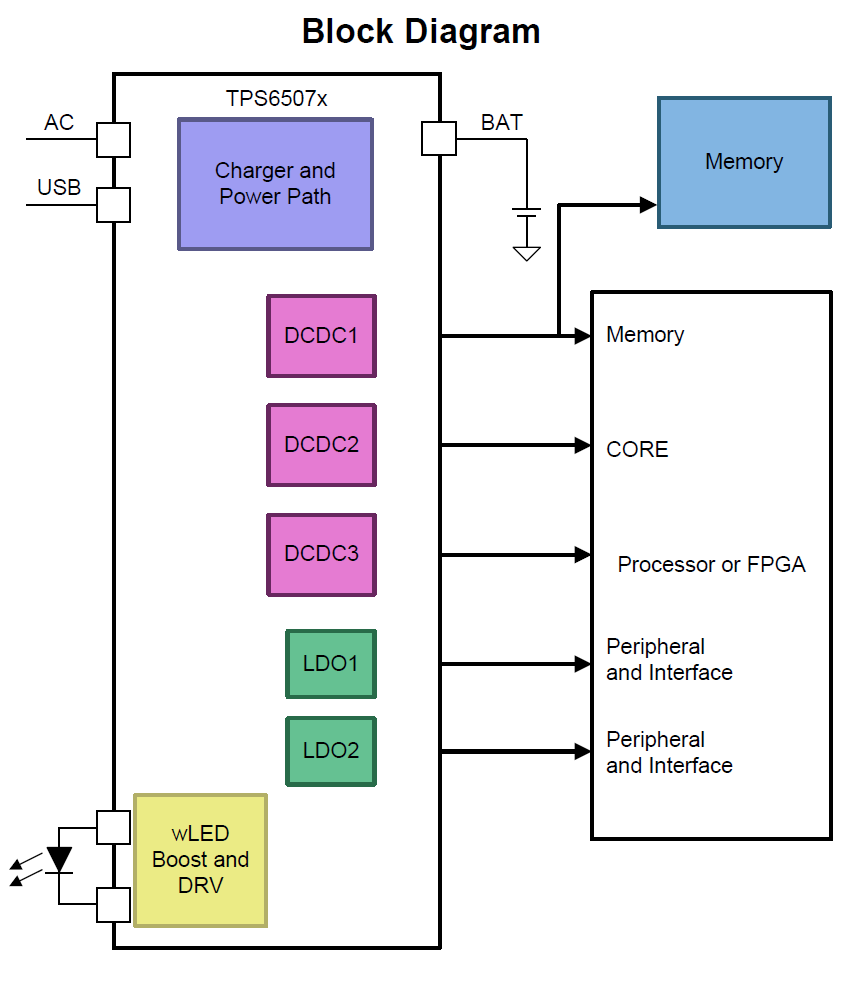
\includegraphics[width = .9\textwidth]{power_managIC.png}
          \caption{Schematic for TPS65070RSL}
          \label{fig:TPS65070RSL}
          \end{minipage}
          \hspace{5mm}
          \begin{minipage}{.5\textwidth}
          \centering
          \begin{tabular}{llr}
          \toprule
          \textbf{Component type} & \textbf{Name} & \textbf{Qty}\\
          \midrule
          Integrated circuit & & \\
           & Regulator & 7\\
           & Analog IC & 5\\
           & Voltage Detector & 1\\
           & Power Manag. IC & 1\\
          \hline
          Discrete Semiconductor & &\\
           & Diode & 30\\
           & Transistor & 35\\
          \hline
          Passive comp. & &\\
           & Capacitor & 176\\
           & Fuse & 1\\
           & Ferrite Bead & 6\\
           & Inductor & 16\\
           & Resistor & 148\\
          \bottomrule
          \end{tabular}
          \caption{Power supply component list}
          \label{tab:power}
          \end{minipage}
        \end{figure}

        \begin{description}
          \item [Control power IC TPS65070RSL] Is a single chip power solution for portable applications that can be powered through a USB port or directly by a DC voltage from a wall adapter connected to "AC" pin. The module has the following main characteristics:
            \begin{itemize}
              \item 2A output current on the power path;
              \item Thermal regulation;
              \item 3 Step-down converters
                \begin{itemize}
                  \item Fixed-frequency operation at 2.25 MHZ;
                  \item Up to 1.5 A output current;
                  \item Adjustable or fixed output Voltage;
                  \item $2.8V < V_{IN} < 6.3V$
                  \item $19\mu A$ of quiescent current per converter;
                  \item 100\% Duty cycle for lowest dropout;
                \end{itemize}
            \end{itemize}
          A block diagram of the module is represented in figure \autoref{fig:TPS65070RSL}.

          The two inputs to the power path (AC and USB) support the same voltage rating but normally have different current limits (Ac is at the higher limit). If voltage is applied at both inputs and both are enabled AC will be preferred over USB and the device will only be powered from AC. The current at the input is shared between charging the battery and powering the system load; anyway priority is given to the system load. The current is always monitored, so that if the sum of the charging and
          system load currents exceeds the present maximum input current the charging current is reduced automatically \cite{ICpower}.

          \item[The Regulator DC/DC Converter AIC1634GG] The module is a current-mode pulse-width modulation (PWM), step-up DC/DC Converter which, through the N-channel MOSFET, allows for step-up applications with up to 30V output voltage. The high switching frequency (1.4MHz) allows the use of small external components.

          There are several characteristics that can be compared in the module, here we list just two comparisons as examples. The first chart (\autoref{fig:efficiency}), shows how the efficiency of the module varies with the evolution of the output current: it can be seen that its value rapidly saturates for low current values and starts decreasing beyond the 40 mA threshold. The second chart (\autoref{fig:SwFreq}) describes the evolution of the switching frequency over the temperature: differently from the efficiency, the frequency continues to constantly grow with the temperature increase \cite{stepupConv}.

          \autoref{fig:blocchi} shows the block diagram for the module.

          \begin{figure}[h]
            \begin{minipage}{.55\textwidth}
              \centering
              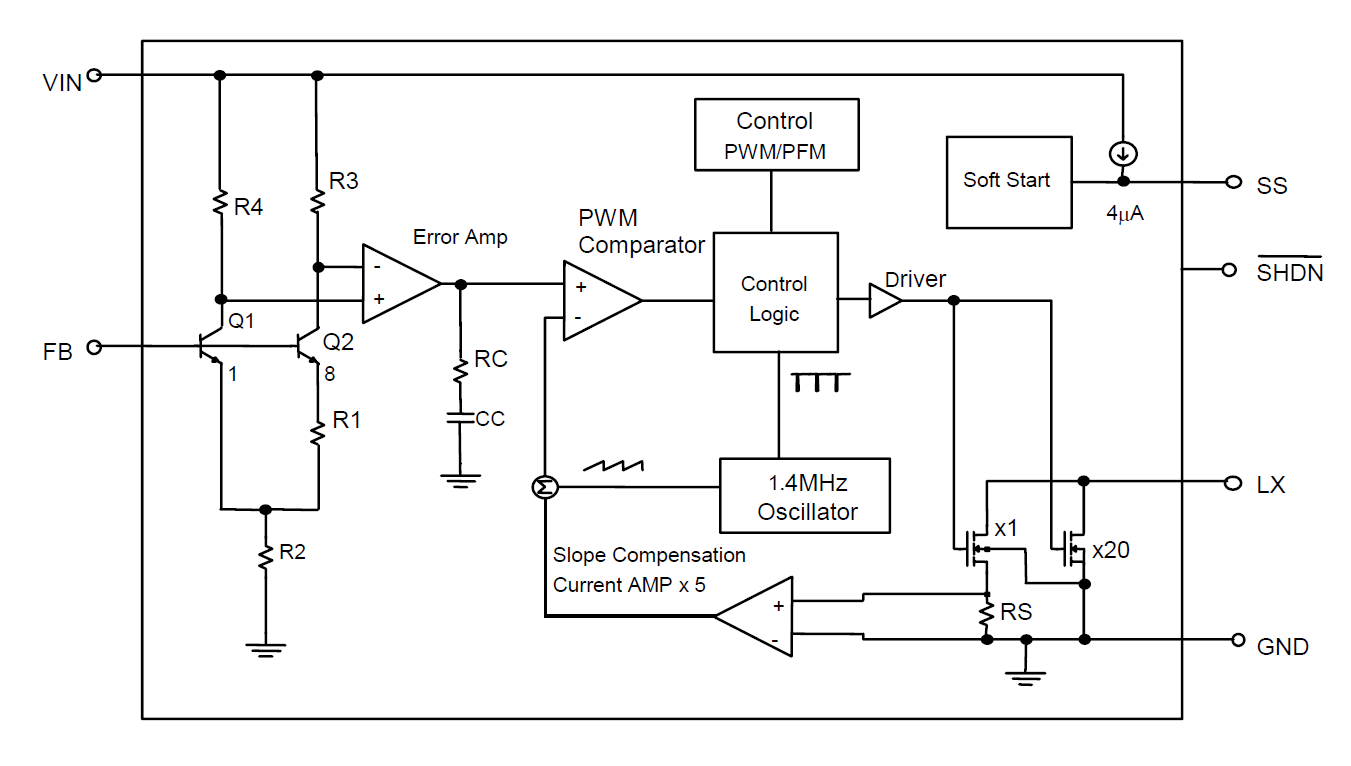
\includegraphics[width = \textwidth]{Schema_blocchi_stepup.png}
              \caption{AIC1634GG block diagram}
              \label{fig:blocchi}
            \end{minipage}
            \hspace{5mm}
            \begin{minipage}{.45\textwidth}
              \centering
              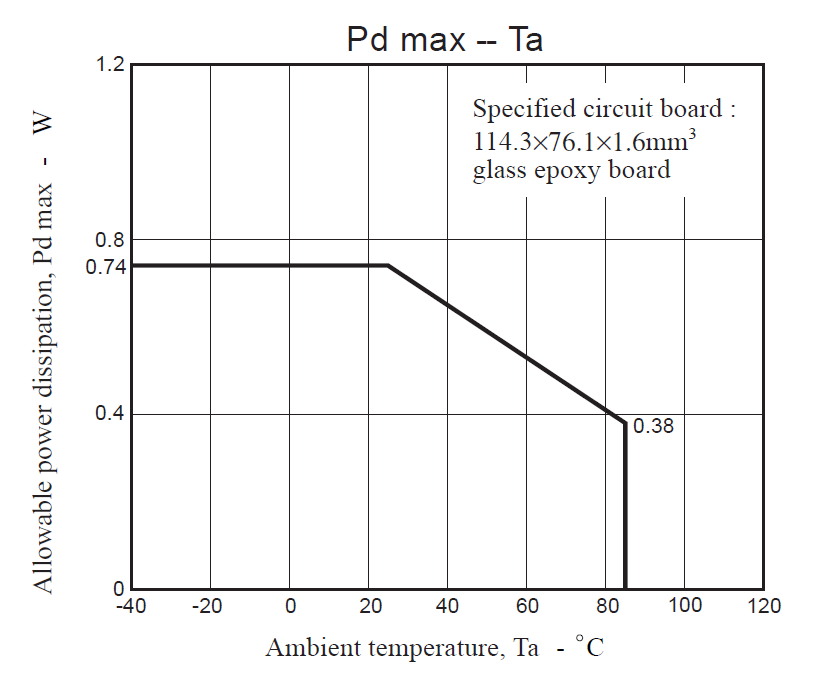
\includegraphics[width = .95\textwidth]{powerVStemp.png}
              \caption{Power constraint over the ambient temperature}
              \label{fig:pdmax}
            \end{minipage}
          \end{figure}

          \begin{figure}
            \begin{minipage}{.5\textwidth}
            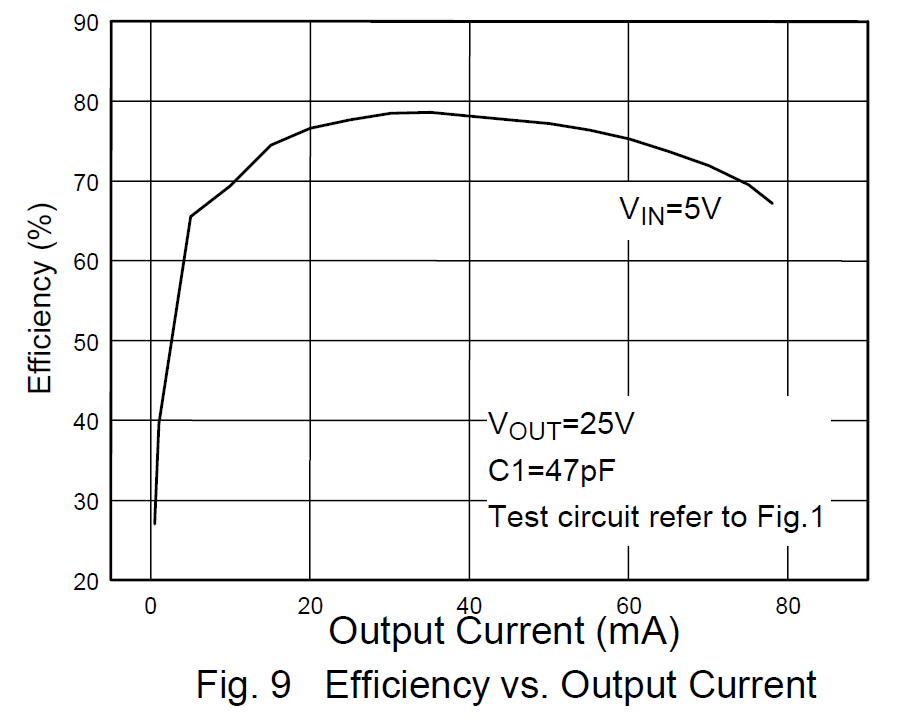
\includegraphics[width = \textwidth]{efficiencyVScurrent.png}
            \caption{}
            \label{fig:efficiency}
            \end{minipage}
            \hspace{5mm}
            \begin{minipage}{.5\textwidth}
            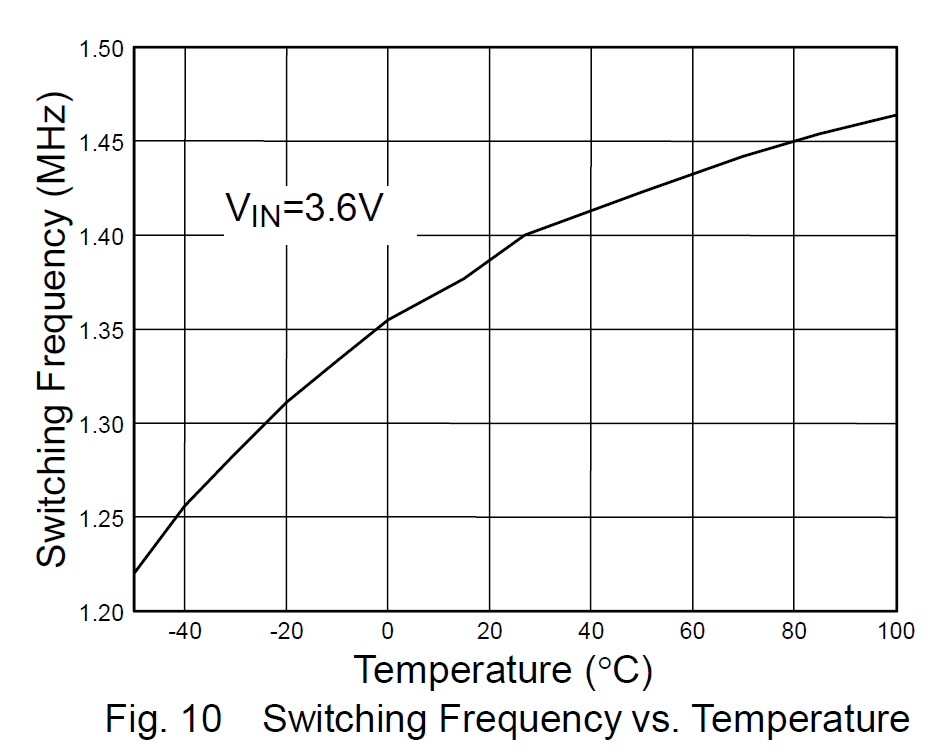
\includegraphics[width = \textwidth]{frequencyVStemp.png}
            \caption{}
            \label{fig:SwFreq}
            \end{minipage}
          \end{figure}

          \item[The switching Regulator DC/DC Controller LV5066V] The last element of this analysis is a step-down switching regulator controller: it has one channel with an operation current of 80$\mu A$ and low power consumption. Also, from \autoref{fig:pdmax} it can be observed the evolution of the allowable power dissipation depending on the ambient temperature: it can be seen how there is a clear power constraint, with a linear decrement of the latter during the interval representing the normal temperature range of a room.

        \end{description}



  \subsection{Wii U gamepad}

\bibliographystyle{IEEEtran}
\bibliography{IEEEabrv,bibliography}

\end{document}
